\documentclass[11pt, letterpaper]{article}

% Essential math and formatting packages
\usepackage[margin=1in]{geometry}
\usepackage{amsmath, amssymb, amsthm}
\usepackage{graphicx}
\usepackage{circuitikz}
\usetikzlibrary{decorations.pathreplacing}
\usepackage{hyperref}
\usepackage{endnotes}
\let\footnote=\endnote

% Add fancyhdr for persistent page footers
\usepackage{fancyhdr}
\pagestyle{fancy}
\fancyhf{} % Clear all default headers and footers
\renewcommand{\headrulewidth}{0pt} % Remove the header line
\fancyfoot[L]{\scriptsize \textbf{Key:} $\omega_{01}$: Initial Waist $|$ $\omega_{02}$: Focused Waist $|$ $z_{01}$: Initial Rayleigh Range $|$ $\alpha$: Magnification $|$ $f$: Focal Length\\~~~~~~~~~ $d_1$: Dist.\ to Lens $|$ $d_2$: Dist.\ to Focus}
\fancyfoot[R]{\thepage}

% Theorem environments for structuring theory
\newtheorem{theorem}{Theorem}[section]
\newtheorem{hypothesis}{Hypothesis}
\newtheorem{definition}{Definition}[section]

% Document Information
\title{\textbf{Theory}\\ \large Gaussian Beam Optics}
\author{Tyler Celotta \\ UAF}
\date{\today}

\begin{document}

\maketitle
\thispagestyle{fancy}
\begin{abstract}
    The purpose of the document is to work through the theory and experimental design for optimizing second-harmonic generation (SHG) at 1064 nm using a periodically poled lithium niobate (PPLN) crystal (50 × 2 × 0.5 mm³). In this document, I define Gaussian beam parameters, including beam waist, Rayleigh range, divergence, and confocal parameter, in order to determine the optimal focusing geometry. The Boyd-Kleinman condition for maximum CW SHG efficiency ($L/b = 2.84$) is a target focused waist of approximately 54.6 µm, but experimental constraints redefines a target of 77–80 µm ($L/b \approx 1.3-1.4$). Starting from a collimated 0.56 mm beam at 1064 nm with a measured divergence of 1.21 mRad, the collimator waist is estimated to be $\omega_{01} \approx 280$ µm, located 6.2 mm behind the collimator face. That being said, the calculated waist radius of roughly 0.279 mm would result in a beam larger than the crystal itself can accommodate. To account for this, I used an ABCD ray-transfer matrix to propigate a beam, constructing two equations relating a chosen lens focal length $f$ to the required lens position $d_{1}$ and image distance $d_{2}$, with magnification $\alpha \approx 0.286$.
\end{abstract}
\section{Experiment Specifics}
\begin{enumerate}
    \item Wavelength: $1064$~nm
    \item Collimator output beam size: $0.56$~mm $\frac{1}{e^2}$ diameter
    \item PPLN crystal: $50 \times 2 \times 0.5$~mm$^3$
    \item Previous best measured output: $57$~mW green, PPLN at $59.5^{\circ}$C
    \item Previous calculated waist: about $45$~$\mu$m
    \item Desired next target: about $77$--$80$~$\mu$m
\end{enumerate}

\section{Definitions and Equations}

\textbf{Beam Diameter ($\frac{1}{e^2}$):} The $\frac{1}{e^2}$ beam diameter captures the diameter where the intensity of the beam drops to $13.53\%$; in other words, $86.47\%$ of the beam intensity lies within the given diameter.

\begin{center}
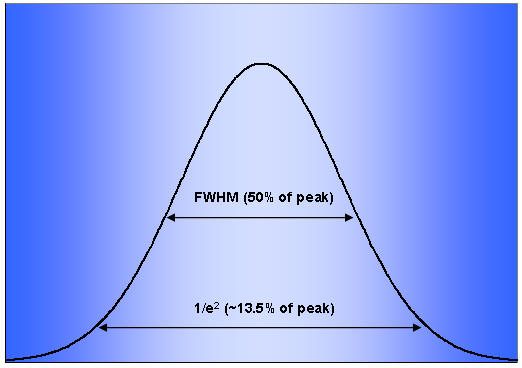
\includegraphics[width=0.25\linewidth]{figures/Picture1en-us.jpg}
\end{center}

\textbf{Beam Waist ($\omega_0$):} The beam waist is the portion of the beam where the radius is minimized, denoted $\omega_0$. The tighter the focus the smaller the waist, but this introduces a large amount of divergence, as seen in the $z$-dependent beam width equation
\begin{equation}\label{omega}
    \omega^2(z)=\omega_0^2\left[1+\left(\frac{\lambda z}{\pi \omega_0^2}\right)^2\right]
\end{equation}
Small waists are achieved by a ``short focal length and a high numerical aperture largely filled by the input beam.''\cite{RPw_0}
\begin{center}
    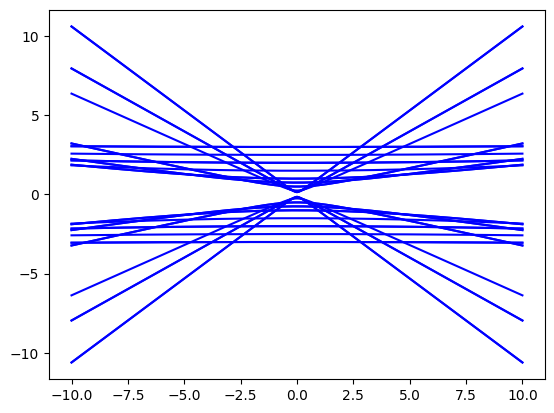
\includegraphics[width=0.4\linewidth]{figures/download.png}
\end{center}

\textbf{Radius of Curvature ($R_g$):} The radius of curvature is defined by Eq.~\ref{roc}. At its boundaries, $\lim_{z\to 0} R_g(z)=\infty$ where the wavefront is perfectly flat and acts like a section of a circle with infinite radius, and $\lim_{z\to\infty}R_g(z)=z$ where the wavefront averages out to a radius equal to the distance from the waist.
\begin{equation}\label{roc}
R_g(z) = z\left[1 + \left(\frac{\pi \omega_0^2}{\lambda z}\right)^2\right]
\end{equation}

\textbf{Rayleigh Range ($z_0$):} The Rayleigh range is the distance at which the cross-sectional area of the beam is no more than twice that of the beam waist, ensuring at least $50\%$ of the beam is retained.\cite{RPz_0}
\begin{equation}\label{z_0}
z_0=\frac{\pi \omega_0^2}{\lambda}
\end{equation}

\textbf{Beam Divergence ($\theta$):} The beam divergence is the slope of the linear component of beam expansion (the far-field expansion), measured as a half-angle dependent on the wavelength and inversely on the waist:
\begin{equation}\label{theta}
    \theta=\frac{\lambda}{\pi \omega_0}
\end{equation}
\begin{center}
    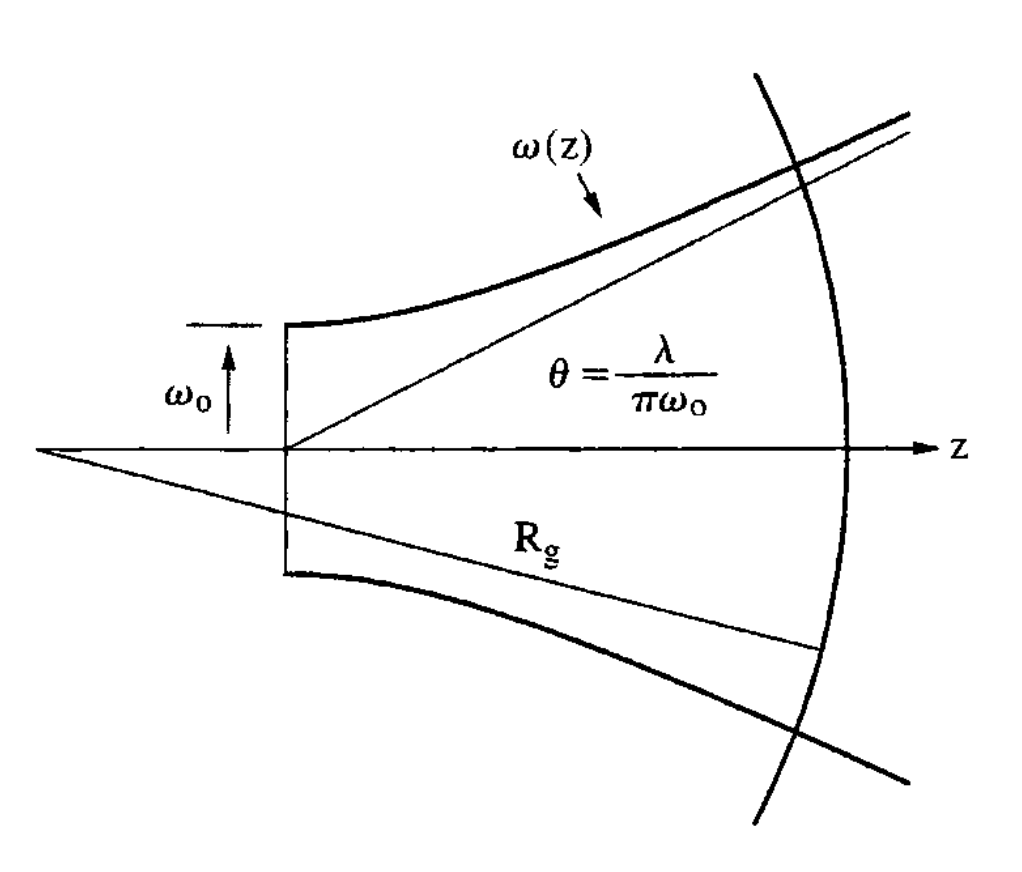
\includegraphics[width=0.3\linewidth]{figures/Screenshot 2026-06-02 at 13.18.55.png}
\end{center}

\textbf{Confocal Parameter ($b$):} The confocal parameter uses the Rayleigh range to quantify the useful depth of focus---it is ``the total length of the focused region around the beam waist.''\cite{RPz_0}

\textbf{Boyd--Kleinman Focusing:}
$h = 1.068$ at $L/b = 2.84$~\cite{boyd};
$h = 1.066$ at $L/b = 2.81$~\cite{hcp}.
Here $h$ is the conversion efficiency, $L$ is the crystal length, and $b = 2z_0$ is the confocal parameter. We work backwards from these values to find the optimal waist; see Section~\ref{sec:bk}.

\footnote{Wikipedia entry: Second-harmonic generation (SHG), also known as frequency doubling, is the lowest-order wave-wave nonlinear interaction that occurs in various systems, including optical, radio, atmospheric, and magnetohydrodynamic systems. As a prototype behavior of waves, SHG is widely used, for example, in doubling laser frequencies. SHG was initially discovered as a nonlinear optical process in which two photons with the same frequency interact with a nonlinear material, are ``combined'', and generate a new photon with twice the energy of the initial photons (equivalently, twice the frequency and half the wavelength), conserving the coherence of the excitation. It is a special case of two-photon sum-frequency generation, and more generally of harmonic generation.}

\footnote{\textbf{Phase-matching:} For sum-frequency generation to occur efficiently, phase-matching conditions must be satisfied: $\hbar k_{3}\approx \hbar k_{1}+\hbar k_{2}$, where $k_{1},k_{2},k_{3}$ are the angular wavenumbers of the three waves travelling through the medium. (This equation resembles conservation of momentum.) The sum-frequency generation becomes more efficient as this condition is satisfied more precisely.}

\section{Calculations}

\subsection{Initial Beam Parameters}

\textit{Starting from a 0.56~mm $1/e^2$ beam diameter at 1064~nm, what are the approximate Gaussian beam parameters?}

Using Eq.~\ref{z_0}:\footnote{In this calculation I assume the full beam diameter $2\omega_{01}=0.56$~mm because the beam emerges from a collimator. This assumes the beam waist may be located a short distance away from the collimator face, as noted in \cite{column}: ``The purpose of a beam collimator is essentially to transform a strongly diverging light beam into a collimated beam, i.e., a beam where light propagates essentially only in one direction, and the beam divergence is weak. The output beam may have its beam waist close to the output aperture, or a mild focus somewhat away from it.''}
$$z_{01}=\frac{\pi \omega_{01}^2}{\lambda}=\frac{\pi\cdot (0.00028)^2}{1.064\times10^{-6}}\approx 0.23149\text{ m}\approx 23.15\text{ cm}$$
This results in $L/b = 0.108$, far from the Boyd--Kleinman optimum.

Using Eq.~\ref{theta}:
$$\theta=\frac{\lambda}{\pi \omega_{01}}=\frac{1.064\times10^{-6}}{\pi \cdot 0.00028}\approx 1.210\times10^{-3}\text{ rad}$$

\subsection{Boyd--Kleinman Focusing Targets}
\label{sec:bk}

\subsubsection{Optimum: $L/b = 2.84$ \cite{boyd}}

\textit{Given $L/b=2.84$ and $L=50$~mm.}
$$b=\frac{L}{2.84}=\frac{0.05}{2.84}~\text{m}$$
Using Eq.~\ref{z_0}:
$$\frac{0.05}{2.84}=b=2z_{02}=\frac{2\pi \omega_{02}^2}{\lambda}
\quad\Rightarrow\quad
\omega_{02}=\sqrt{\frac{1064\times10^{-9}\cdot 0.05}{2\pi\cdot 2.84}}\approx 54.602~\mu\text{m}$$

\subsubsection{Optimum: $L/b = 2.81$ \cite{hcp}}

\textit{Given $L/b=2.81$ and $L=50$~mm.}
$$b=\frac{L}{2.81}=\frac{0.05}{2.81}~\text{m}$$
Using Eq.~\ref{z_0}:
$$\frac{0.05}{2.81}=b=2z_{02}=\frac{2\pi \omega_{02}^2}{\lambda}
\quad\Rightarrow\quad
\omega_{02}=\sqrt{\frac{1064\times10^{-9}\cdot 0.05}{2\pi\cdot 2.81}}\approx 54.892~\mu\text{m}$$

\subsubsection{Conservative rule of thumb: $L/b = 1$ \cite{PPLN}}
\footnote{``In general, a good rule of thumb is that the spot size should be chosen such that the Rayleigh range is half the length of the crystal.'' If $z_{02}=L/2$, then $b=2z_{02}=L$, so $L/b=1$.}

\textit{Given $L/b=1$ and $L=50$~mm.}
$$b=L=0.05~\text{m}$$
Using Eq.~\ref{z_0}:
$$0.05=b=2z_{02}=\frac{2\pi \omega_{02}^2}{\lambda}
\quad\Rightarrow\quad
\omega_{02}=\sqrt{\frac{1064\times10^{-9}\cdot 0.05}{2\pi}}\approx 92.017~\mu\text{m}$$

\subsubsection{Working Backwards from Target Waists}

To recover a desired $\omega_{02}$, we solve for $\xi \equiv L/b$:

\begin{enumerate}
    \item $\omega_{02}=45~\mu$m:
$$\xi=\frac{1064\times10^{-9}\cdot 0.05}{2\pi\cdot(45\times10^{-6})^2}\approx 4.181$$
This ratio is too large (waist too tight), leading to excessive diffraction and reduced efficiency.

    \item $\omega_{02}=77~\mu$m:
$$\xi=\frac{1064\times10^{-9}\cdot 0.05}{2\pi\cdot(77\times10^{-6})^2}\approx 1.428$$
Within the proper range.

    \item $\omega_{02}=80~\mu$m:
$$\xi=\frac{1064\times10^{-9}\cdot 0.05}{2\pi\cdot(80\times10^{-6})^2}\approx 1.323$$
Within the proper range.
\end{enumerate}

\subsection{Collimator Waist Estimation}
\label{sec:colwaist}

\textit{Repeating the analysis without assuming the beam waist is at the collimator face.}\footnote{Note: 1.21~mRad was a measured value, substantially lower than the spec sheet value of approximately 5~mRad.}

\begin{enumerate}
    \item Using Eq.~\ref{theta} to recover the waist from the measured divergence:
$$\omega_{01}=\frac{\lambda}{\pi\theta}=\frac{1.064\times10^{-6}}{\pi\cdot 0.00121}\approx 279.9~\mu\text{m}$$

    \item Using the beam propagation equation (Eq.~\ref{w(z)}, from Eq.~2-27 in \cite{Osche}):
\begin{equation}\label{w(z)}
    \omega^2(z)=\omega_{01}^2\left[1+\left(\frac{\lambda z}{\pi \omega_{01}^2}\right)^2\right]
\end{equation}
Solving for $z$:
$$\frac{\omega^2(z)}{\omega_{01}^2}-1=\left(\frac{\lambda z}{\pi \omega_{01}^2}\right)^2
\quad\Rightarrow\quad
z=\pm\left(\sqrt{\frac{\omega^2(z)}{\omega_{01}^2}-1}\right)\frac{\pi \omega_{01}^2}{\lambda}$$
Setting $\omega(z)=0.00028$~m (the $1/e^2$ radius at the collimator aperture):
$$z\approx\pm\left(\sqrt{\frac{(0.00028)^2}{(0.0002799)^2}-1}\right)\frac{\pi\cdot(0.0002799)^2}{1.064\times10^{-6}}\approx \pm 6.184\text{ mm}$$
The waist is located approximately 6.2~mm \emph{behind} the collimator face.\footnote{The following calculations were made under the (incorrect) assumption of a waist radius of 45~$\mu$m rather than the updated 279.9~$\mu$m derived here.\\
\begin{center}
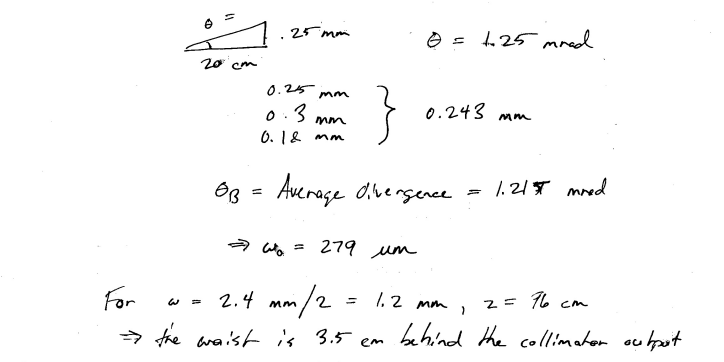
\includegraphics[width=0.5\linewidth]{figures/ss1.png}
\end{center}}

    \item Recalculating the Rayleigh range with the corrected waist:
$$z_{01}=\frac{\pi \omega_{01}^2}{\lambda}=\frac{\pi\cdot(2.799\times10^{-4})^2}{1.064\times10^{-6}}\approx 23.132\text{ cm}$$

    \item Because the beam waist $\omega_{01}\approx 280~\mu$m is the \emph{minimum} radius of the laser, the beam can only diverge from that point and would ``scrape'' the inside of the PPLN crystal. A focusing lens is therefore required.
\end{enumerate}

\subsection{Lens Selection}
\label{sec:lens}

\begin{enumerate}
    \item The magnification relation from \cite{edmund}:
\begin{equation}\label{M}
    \omega_{02}=\alpha\cdot\omega_{01}
    \quad\Rightarrow\quad
    \alpha=\frac{\omega_{02}}{\omega_{01}}
\end{equation}

    \item The lens-placement formula from \cite{edmund}:
\begin{equation}\label{18}
    \alpha = \frac{f}{\sqrt{(|d_1| - f)^2 + z_{01}^2}}
\end{equation}
Solving for $|d_1|$:
$$\alpha^2\bigl[(|d_1|-f)^2+z_{01}^2\bigr]=f^2
\quad\Rightarrow\quad
|d_1|=\sqrt{\left(\frac{f}{\alpha}\right)^2-z_{01}^2}+f$$

    \item Image-distance formula from \cite{edmund}:
\begin{equation}\label{22}
    d_2 = f + \alpha^2(d_1 - f)
\end{equation}

    \item \textbf{Numerical values.} With $\omega_{02}=80~\mu$m and $\omega_{01}=279.9~\mu$m:
$$\alpha=\frac{80}{279.9}\approx 0.28582,\qquad z_{01}\approx 0.23132\text{ m}$$
For a focal length $f$ chosen in the lab:
$$d_1 = \sqrt{\left(\frac{f}{0.28582}\right)^2-(0.23132)^2}+f,
\qquad
d_2 = f + (0.28582)^2(d_1-f)$$

    \item \textbf{Derivation of equations used above} Starting from \cite{Osche}:
\begin{equation}\label{complex}
    \frac{1}{q_1} = \frac{1}{R_{g}} - i\frac{\lambda}{\pi \omega_{01}^2}
\end{equation}
where $R_g$ is the radius of curvature of the input beam. Taking the limit $R_g\to\infty$ (collimated input):
$$q_1 = i\frac{\pi \omega_{01}^2}{\lambda}=iz_{01}$$
The ABCD ray-transfer matrix for free-propagation $d_1$, thin lens $f$, then free-propagation $d_2$ is:
$$\begin{pmatrix} A & B \\ C & D \end{pmatrix}
= \begin{pmatrix} 1 & d_2 \\ 0 & 1 \end{pmatrix}
  \begin{pmatrix} 1 & 0 \\ -\frac{1}{f} & 1 \end{pmatrix}
  \begin{pmatrix} 1 & d_1 \\ 0 & 1 \end{pmatrix}
=\begin{pmatrix} 1 - \frac{d_2}{f} & d_1 + d_2 - \frac{d_1 d_2}{f} \\ -\frac{1}{f} & 1 - \frac{d_1}{f} \end{pmatrix}$$
so $A=1 - \frac{d_2}{f}$, $B=d_1 + d_2 - \frac{d_1 d_2}{f}$, $C=-\frac{1}{f}$, $D=1 - \frac{d_1}{f}$.

The $q$-parameter transforms as (Eq.~\ref{q2} from \cite{Osche}):
\begin{equation}\label{q2}
q_2 = \frac{A q_1 + B}{C q_1 + D}
\end{equation}
Substituting $q_1=iz_{01}$:
$$q_2=\frac{\left(1 - \frac{d_2}{f}\right)iz_{01} + \left(d_1 + d_2 - \frac{d_1 d_2}{f}\right)}{\left(-\frac{1}{f}\right)iz_{01} + \left(1 - \frac{d_1}{f}\right)}$$
Multiplying numerator and denominator by the complex conjugate of the denominator,
$\left(1 - \frac{d_1}{f}\right)+i\left(\frac{z_{01}}{f}\right)$:

\medskip
\textit{Real part:}
$$\operatorname{Re}(q_2)=\frac{-\left(1-\frac{d_2}{f}\right)\left(\frac{z_{01}^2}{f}\right)+\left(d_1+d_2-\frac{d_1d_2}{f}\right)\left(1-\frac{d_1}{f}\right)}{\left(\frac{z_{01}}{f}\right)^2+\left(1-\frac{d_1}{f}\right)^2}$$
$$=\frac{d_2\left[\left(1 - \frac{d_1}{f}\right)^2 + \frac{z_{01}^2}{f^2}\right] + d_1\left(1 - \frac{d_1}{f}\right) - \frac{z_{01}^2}{f}}{\left(\frac{z_{01}}{f}\right)^2+\left(1-\frac{d_1}{f}\right)^2}$$
$$= d_2 + \frac{d_1\left(1 - \frac{d_1}{f}\right) - \frac{z_{01}^2}{f}}{\left(\frac{z_{01}}{f}\right)^2+\left(1-\frac{d_1}{f}\right)^2}$$

\medskip
\textit{Imaginary part:}
$$\operatorname{Im}(q_2)=\frac{z_{01}\left[\left(1-\frac{d_1}{f}-\frac{d_2}{f}+\frac{d_1d_2}{f^2}\right)+\left(\frac{d_1}{f}+\frac{d_2}{f}-\frac{d_1d_2}{f^2}\right)\right]}{\left(\frac{z_{01}}{f}\right)^2+\left(1-\frac{d_1}{f}\right)^2}
=\frac{z_{01}}{\left(\frac{z_{01}}{f}\right)^2+\left(1-\frac{d_1}{f}\right)^2}$$

\medskip
\textit{Full expression:}
$$q_2=\left[d_2 + \frac{d_1\!\left(1 - \frac{d_1}{f}\right) - \frac{z_{01}^2}{f}}{\left(\frac{z_{01}}{f}\right)^2+\left(1-\frac{d_1}{f}\right)^2}\right]+i\left[\frac{z_{01}}{\left(\frac{z_{01}}{f}\right)^2+\left(1-\frac{d_1}{f}\right)^2}\right]$$

Setting the real part to zero to satisfy the waist condition: $\lim\limits_{z\to 0}\frac{1}{R_g(z)}=0$ results in
$$d_2 = \frac{f\!\left[(d_1-f)^2 + z_{01}^2\right] + f^2(d_1-f)}{(d_1-f)^2+z_{01}^2}
= f + \frac{f^2(d_1-f)}{(d_1-f)^2+z_{01}^2}$$
$$d_2 = f + \alpha^2(d_1 - f)$$
proving Eq.~\ref{22}, where $\alpha^2 = \frac{f^2}{(d_1-f)^2+z_{01}^2}$ follows Eq.~\ref{18}.
\end{enumerate}

\section{Use Case}

\textbf{PPLN:}\footnote{Periodically poled lithium niobate (PPLN) is a lithium niobate crystal that switches polarity in a periodic fashion and is used for achieving quasi-phase-matching in nonlinear optics.} To get the most out of our PPLN crystals, four key aspects must be considered:

\begin{enumerate}
    \item \textbf{Crystal Length}
    \begin{enumerate}
        \item No special action required at this stage.
    \end{enumerate}

    \item \textbf{Polarization}
    \begin{enumerate}
        \item The input light must be e-polarized, i.e.\ the polarization must be aligned with the dipole moment of the crystal. This is accomplished by aligning the polarization axis of the light parallel to the thickness of the crystal.\cite{PPLN}
    \end{enumerate}

    \item \textbf{Focusing and the Optical Arrangement}
    \begin{enumerate}
        \item For SHG with CW lasers, the Boyd--Kleinman result shows that optimum conversion efficiency is achieved when $L/b = 2.84$.\cite{PPLN}
    \end{enumerate}

    \item \textbf{Temperature and Period}
    \begin{enumerate}
        \item The crystal is manufactured with periodic stripes of alternating polarity with a spacing called the poling period. This quasi-phase-matched arrangement allows the harmonic power to build up continuously.
        \item The effective poling period can be tuned by changing the crystal temperature, which causes thermal expansion or contraction.
        \item Note: The refractive index of the crystal also changes with temperature.
        \item The output intensity follows a $\operatorname{sinc}^2$ curve (shown below), defining the temperature acceptance bandwidth.
        \begin{center}
            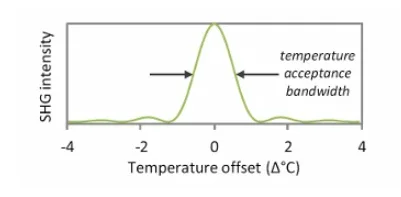
\includegraphics[width=0.5\linewidth]{TP-Graph-4.png.png}
        \end{center}
        \item Acceptance bandwidth is inversely proportional to crystal length.
        \item The optimum temperature can be found by heating the crystal to $20^{\circ}$C above the calculated phase-matching temperature, then allowing it to cool while monitoring the generated output power.\cite{PPLN}
    \end{enumerate}
\end{enumerate}

\begin{figure}[h]
    \centering
    \resizebox{\textwidth}{!}{
    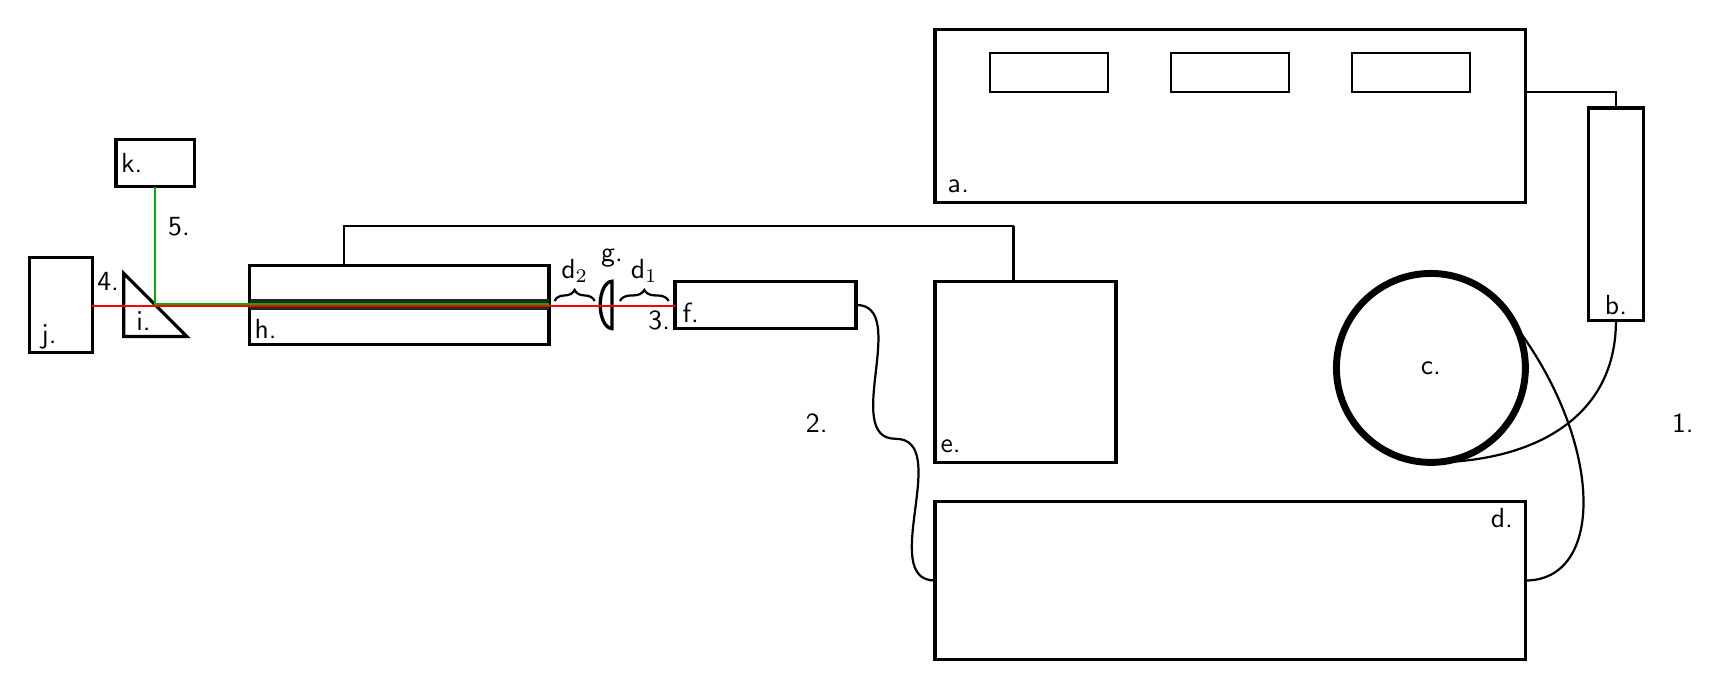
\begin{tikzpicture}[font=\sffamily]
        
        % ---------------------------------------------------
        % 1. Boxes and Shapes
        % ---------------------------------------------------
        
        % i. Left box
        \draw[very thick] (0, -0.6) rectangle (0.8, 0.6);
        \node at (0.25, -0.4) {j.};
        
        % h. Prism / Beam Splitter (Right-angled triangle)
        % Hypotenuse acts as a 45-degree mirror for the green laser
        \draw[very thick] (1.2, 0.4) -- (1.2, -0.4) -- (2.0, -0.4) -- cycle;
        \node at (1.45, -0.2) {i.};
        
        % j. Top box
        \draw[very thick] (1.1, 1.5) rectangle (2.1, 2.1);
        \node at (1.3, 1.8) {k.};
        
        % g. Long box
        \draw[very thick] (2.8, -0.5) rectangle (6.6, 0.5);
        \node at (3.0, -0.3) {h.};
        
        % Dark inner channel in g
        \draw[line width=4pt, black!85] (2.8, 0) -- (6.6, 0); 
        
        % e. Lens (Plano-convex facing left)
        % Arc draws the curved left side, flat side is on the right
        \draw[very thick] (7.4, -0.3) arc (270:90:0.15 and 0.3) -- cycle;
        \node at (7.4, 0.6) {g.}; % Moved up to avoid brace overlap
        
        % f. Small middle box
        \draw[very thick] (8.2, -0.3) rectangle (10.5, 0.3);
        \node at (8.4, -0.1) {f.};
        
        % e. Square box (lower middle)
        \draw[very thick] (11.5, -2.0) rectangle (13.8, 0.3);
        \node at (11.7, -1.8) {e.};
        
        % a. Large Top Right Box
        \draw[very thick] (11.5, 1.3) rectangle (19.0, 3.5);
        \node at (11.8, 1.5) {a.};
        % Inner rectangles inside a.
        \draw[thick] (12.2, 2.7) rectangle (13.7, 3.2);
        \draw[thick] (14.5, 2.7) rectangle (16.0, 3.2);
        \draw[thick] (16.8, 2.7) rectangle (18.3, 3.2);
        
        % c. Thick Circle / Fiber Spool
        \draw[line width=2.5pt] (17.8, -0.8) circle (1.2cm);
        \node at (17.8, -0.8) {c.};

        % d. Large Bottom Right Box
        \draw[very thick] (11.5, -4.5) rectangle (19.0, -2.5);
        \node at (18.7, -2.7) {d.};
        
        % b. Vertical Box
        \draw[very thick] (19.8, -0.2) rectangle (20.5, 2.5);
        \node at (20.15, 0) {b.};


        % ---------------------------------------------------
        % 2. Optical Paths (Red and Green Lines)
        % ---------------------------------------------------
        
        % Red Path (Straight through from i to f)
        % Shifted minutely down so it forms a two-tone line with the green laser
        \draw[red, thick] (0.8, -0.015) -- (8.2, -0.015);

        % Green Path (Down from j, bounces right off h)
        % Shifted minutely up so both colors are visible overlapping the black channel
        \draw[green!70!black, thick] (1.6, 1.5) -- (1.6, 0.015) -- (6.6, 0.015);


        % ---------------------------------------------------
        % 3. Electrical / Fiber Connections (Black Wires)
        % ---------------------------------------------------
        
        % Wire from g up and splitting into a and square e
        \draw[thick] (4.0, 0.5) -- (4.0, 1.0) -- (12.5, 1.0);
        \draw[thick] (12.5, 1.0) -- (12.5, 0.3); % Down to box e
        
        % Wavy Wire 2 from f to d
        \draw[thick] (10.5, 0) to[out=0, in=180] (11.0, -1.7) to[out=0, in=180] (11.5, -3.5);
        
        % Wire from a to b
        \draw[thick] (19.0, 2.7) -- (20.15, 2.7) -- (20.15, 2.5);
        
        % Fiber Loop 1 (b -> spool c -> d)
        % Entering spool area from bottom of b
        \draw[thick] (20.15, -0.2) .. controls (20.15, -1.5) and (19.0, -2.0) .. (17.8, -2.0);
        % Leaving spool area to d, crossing the previous curve
        \draw[thick] (18.9, -.3) .. controls (20.0, -1.8) and (20.0, -3.5) .. (19.0, -3.5);


        % ---------------------------------------------------
        % 4. Labels, Numbers, and Braces
        % ---------------------------------------------------
        
        % Distances (Above gaps)
        \draw[thick, decorate, decoration={brace, amplitude=4pt}] (6.67, 0.05) -- (7.18, 0.05) node[midway, above=3pt] {d$_2$};
        \draw[thick, decorate, decoration={brace, amplitude=4pt}] (7.5, 0.05) -- (8.12, 0.05) node[midway, above=3pt] {d$_1$};
        
        % Numbers
        \node at (1.0, 0.3) {4.};
        \node at (1.9, 1.0) {5.};
        \node at (8.0, -0.2) {3.};
        \node at (10.0, -1.5) {2.};
        \node at (21.0, -1.5) {1.};

    \end{tikzpicture}
    }
    \vspace{0.5cm} % Adds a little breathing room
    \renewcommand{\arraystretch}{1.2} % Spaces out the rows slightly
    \small % Reduces font size for the legend
    \begin{tabular}{@{}ll | ll@{}}
        \textbf{1.} & 1064\,nm laser beam (fiber)           & \textbf{a.} & Laser power source \\
        \textbf{2.} & Amplified 1064\,nm laser beam (fiber) & \textbf{b.} & 1064\,nm laser \\
        \textbf{3.} & 1064\,nm laser                        & \textbf{c.} & Spool of fiber \\
        \textbf{4.} & 1064\,nm laser                        & \textbf{d.} & Amplifier \\
        \textbf{5.} & 532\,nm laser                         & \textbf{e.} & Crystal warmer \\
                    &                                       & \textbf{f.} & Collimator \\
                    &                                       & \textbf{g.} & Focusing lens \\
                    &                                       & \textbf{h.} & Crystal housing \\
                    &                                       & \textbf{i.} & Beam splitter \\
                    &                                       & \textbf{j.} & Beam stopper \\
                    &                                       & \textbf{k.} & Power meter \\
    \end{tabular}
    \vspace{0.3cm}
    \caption{Experimental setup and component legend.} 
\end{figure}
\newpage
\section{Operating Instructions}
\subsection{Prerequisites}
\begin{itemize}
    \item Ensure curtains are closed and laser indicator is on outside the lab.
    \item Take off all jewlery and don appropriate laser safety goggles.
    \item Verify the beam path is clear of obstructions and that all optical components are securely mounted.
    \item Verify the power meter is aligned and is propperly rated for the expected power levels, default to 500~mW.
    \item Intiaite approprite music... a good fall back is Led Zepplin, Black Sabith, or AC/DC. 
\end{itemize}

\subsection{Diode Initialization}
\begin{enumerate}
    \item Turn on the diode, ilx, it is located on the top shelf on the far right, it is blue.
    \item Check the current and temperature settings on the diode controller, Temp should be $19.5^{\circ}$C and Current should be $165$~mA.
    \item Turn on the temperature via TEC controler, push ON.
    \item Turn on the current via the controller, push ON.
\end{enumerate}
\subsection{PPLN Initialization}
\begin{enumerate}
    \item Verify HCP is set to 59.5$^{\circ}$C, then turn on the PPLN temperature controller.
\end{enumerate}
\begin{center}
    \textbf{PUT ON SAFETY GOGGLES BEFORE PROCEEDING FURTHER}
\end{center}
\subsection{Amplifier Initialization}
\begin{enumerate}
    \item Turn on the amplifier, but leave the key switched off for now.
    \item Verify the amplifier settings: the current should be set to $20$~mA.
    \item Turn on the amplifier key switch, then wait for system to boot through serial number and loading screens.
    \item Turn on the amplifier output by turning the dial to highlight \textit{START}, then push the dial in.
\end{enumerate}

\subsection{How to Shut Down the Laser System}
\begin{enumerate}
    \item Turn the key to off on the amplifier and then shut it down.
    \item Flip the current off and then the TEC peltier device off.
    \item Turn off the crystal heater
\end{enumerate}
\subsection{Troubleshooting}
Placeholder for troubleshooting instructions.
\newpage
\theendnotes
\bibliographystyle{plain}
\bibliography{theory}

\end{document} 